\chapter{Background}
%labels will help you to reference to certain images, tables, chapters, section, and so on...
\label{background}

DELETEME: This chapter will cover all of your background information and related work. Background and related work are directly related to your thesis. Please do not place irrelevant content here which is a common mistake. Citing will be handled in the appendices.

DELETEME: Background represents underlaying knowledge that is required to understand your work. The expected knowledge level of your readers can be set to the one of a bachelor or master student who just finished his studies (depending on what kind of thesis you are writing). This means that you do not need to describe how computers work, unless your thesis topic is about this. Everything that an avarage alumni from your field of studies should now does not need to be described. It turn, background information that is very complex and content-wise very near to you problem, can be placed in the main parts. Everyting else should be written here. Note: it is important to connect each presented topic to your thesis. E.g. if you present the ISO/OSI layer model you should also write that this is needed to understand the protocols you plan to develop in the main parts.

DELETEME: Related work respresents results from work that handled the same or a similar problem that you are addressing. This work might have used a different approach or might not have been that successful. Finding a paper / work that solved your problem in the same way you were planning to do is not good and you should contact your supervizor for solving this issue. Again, each paper / work has to be connected to your approach: other papers might have not chosen an optimal solution; they might not have been taking care of essential aspects; they might have chosen a different approach and you believe, yours will work better ...

%###################################################################################
%###################### Topic A             ########################################
%###################################################################################
\section{Topic 1}

%###################################################################################
%###################### Topic B             ########################################
%###################################################################################
\section{Topic 2}

%###################################################################################
%###################### Topic C             ########################################
%###################################################################################
\section{Gated recurrent unit}
The artifical neural network (ANN) of the navigation method of this thesis
integrates the PyTorch implementation\footnote{
    \url{https://pytorch.org/docs/stable/generated/torch.nn.GRU.html}, visited on 09/07/2022
}
of the gated recurrent unit (GRU)
with the objective to involve temporal comprehension in
the navigation decision making.
The GRU,
published in 2014 by Cho et al. \cite{Cho2014},
is a variant of the ANN class of recurrent neural networks (RNN).
This section shortly introduces the RNN class
and justifies the design choice for the GRU
in light of standard RNNs and the more prevalent long short-term memory (LSTM).
Moreover, it provides an insight into
the mechanisms of the GRU that make temporal comprehension available
as well as the loss backpropagation through time at the training of the GRU.

\paragraph*{Recurrent neural networks} ${}$\\
RNNs contrasts with classical feedforward ANNs,
which forward information exclusively towards subsequent layers,
by featuring dynamic properties 
that stem from the implementation of feedback connections
\cite{Hu2008} (see fig. \ref{fig:rnn_folded}).
As previously infered states re-enter the network,
the output of an RNN depends not only on the 
current but also on prior inputs.
In this sense, an RNN is qualified to process and reason on
entire sequences of data points.
In case of time-series data, this can be interpreted as 
temporal comprehension and memory \cite{ICE2020}.
RNNs are trained on sequential data with
backpropagation through time (BPTT) \cite{pascanu2013difficulty}
which is basically the application of standard backpropagation
(e.g., \cite{Rojas1996})
on the unfolded representation of the RNN.
The unfolded representation exhibits a layer for
each data point in the given input sequence 
(see figure \ref{fig:rnn_unfolded})
and can be construed as a feedforward ANN
that shares its trainable parameters across its layers.
The longer the input sequences,
the deeper the unfolded representation of an RNN becomes.
The training of RNNs on long sequences
is hence prone to the vanishing gradient problem \cite{hochreiter1991untersuchungen},
which manifests itself in the premature slowdown or standstill 
of the convergence of the RNN.
As a result, it is difficult to
teach standard RNNs to
make connections to information of inputs deep in the past
\cite{Bengio1994}.


\begin{figure}[h]
    \centering
    \subfloat[
        Folded
    ]{
        \label{fig:rnn_folded}
        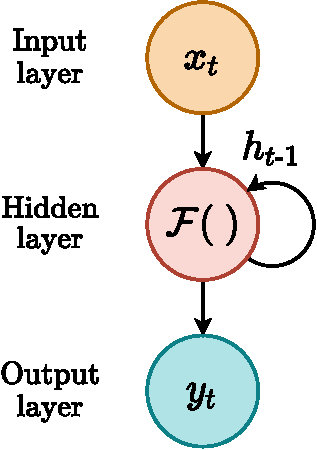
\includegraphics[height=0.35\textwidth]{own/rnn_folded.drawio.pdf}
    }
    \hspace*{2cm}                
    \subfloat[
        Unfolded
    ]{
        \label{fig:rnn_unfolded}
        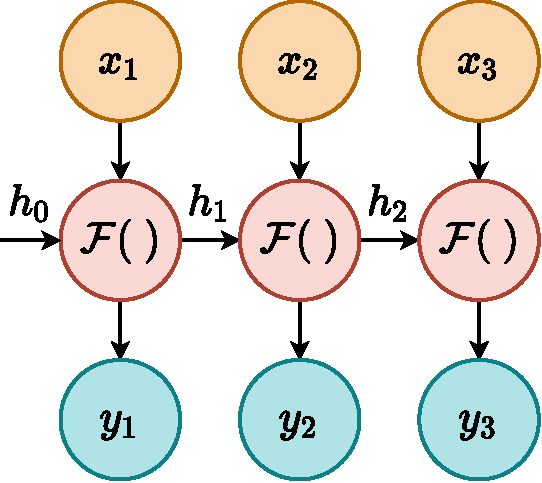
\includegraphics[height=0.35\textwidth]{own/rnn_unfolded.drawio.pdf}
    }
    \caption[
        Folded and unfolded RNN
    ]{
        Folded schematic RNN with a single hidden layer 
        that feeds the previous $h_{t-1}$ 
        (or initial $h_{0}$) state  
        back to the inference at the current time step $t$
        and its time-unfolded representation
        when processing the input of a time-series 
        consisting of the three data points 
        $\left(x_i\right)_{i\in\{1, 2, 3\}}$.

        \label{fig:rnn_folded_unfolded}
    }
\end{figure}

In 1997, Hochreiter and Schmidhuber \cite{Hochreiter1997} introduced
the long short-term memory (LSTM),
which is today's predominant \cite{schmidhuber_2021} RNN variant.
A standard LSTM layer
(see, e.g., the PyTorch implementation\footnote{
    \url{https://pytorch.org/docs/stable/generated/torch.nn.LSTM.html}, visited on 03/07/2022
})
recurrently maintains a cell and a hidden state,
i.e., the layer,
in addition to the current data point of the input sequence,
re-inputs the fed back cell and hidden state
outputted at the previous sequential step.
%The cell state is able to 
%conserve its information content
%over an arbitrary amount of sequential steps \cite{pascanu2013difficulty}.
Furthermore, the LSTM layer implements three gating mechanism
that control the information flow within the layer.
A gating mechanism is basically
the Hadamard product of a state and a gate, which is a vector whose entries 
are within the interval from zero to one. 
Consequently, a gate applied on a state, controls the 
flow of the elements of the state within the range from zero to full flow.
The forget gate of the LSTM layer controls
the flow from the previous to the current cell state.
The input gate controls the flow from the
previous hidden state and the current data point of the input sequence
to the current cell state.
And the output gate controls
the flow from the current cell state to current hidden state.
%All three gates are functions of 
%the previous hidden state and the current element of the input sequence.
%The LSTM integrates a cell
%as well as the input, output and forget gate.
%While the cell conserves its state
%over an arbitrary amount of inferences,
%the three gates determine the information 
%that flows into the cell to update the cell state
%and out of the cell to impact the output.
By this design of recurrent states with gated information flow,
the training of the LSTM is essentially 
robust to the vanishing gradient problem \cite{pascanu2013difficulty}.
As a result, the LSTM is essentially 
more capable of learning to remember long-term dependencies within input sequences
than standard RNNs.




The GRU,
which was proposed 17 years after the LSTM by Cho et al. \cite{Cho2014},
can be seen as a lighter version of the LSTM.
It refrains from the cell state and therewith the output gate
of the LSTM and maintains only a hidden state and two gating mechanisms.
Therewith, the GRU has less trainable parameters than the LSTM
and is less memory efficient during inference.
Nevertheless, it preserves the robustness with respect to the 
vanishing gradient problem that affects most standard RNNs \cite{ICE2020}.
Various empirical studies show that the GRU, compared to the LSTM,
performs equally well or even slightly better.
Greff et al. \cite{Greff2017} evaluated 
the "vanilla" LSTM and the GRU, among other LSTM variants,
on speech and handwritten text recognition
as well as music representation
and could not detect substantial differences in performance.
Chung et al. \cite{Chung2014} applied LSTM and GRU on
raw speech and polyphonic music data and empirically
observed that both performed equally well.
In the comparative study of 
Yin et al. \cite{Yin2017}, 
the GRU slightly outperforms
the LSTM on five of seven
natural language processing tasks.
In the field of algorithm learning, 
Kaiser and Sutskever \cite{Kaiser2015} achieved notedly better results 
with a network based on GRU
than with a network based on LSTM.
In consideration of these findings and the
fact that the GRU has less trainable parameters
and occupies less memory during inference,
the GRU is chosen over the LSTM for the deployment 
in the ANN module of the navigation method of this thesis.




\paragraph*{Inference}$\ $\\
The following presents the mathematics of a single GRU layer during inference
in accordance with the PyTorch implementation\footnote{
    \url{https://pytorch.org/docs/stable/generated/torch.nn.GRU.html}, visited on 09/07/2022
}.
This includes the GRU layer's two gating mechanisms
as well as its computations of the candidate and the hidden state.






Without loss of generality,
let the sequential data to be processed by the GRU layer
be a batch of time series of data points
\begin{equation}
    \left(
        \underline x_t
        \in \mathbb{R}^{N^\text{in}}
    \right)_{
        t \in \left\{
            1, \dots, N^\text{seq}
        \right\}
        ,
        i
    }
    ,\quad
    i \in \left\{
        1, \dots, N^\text{batch}
    \right\}
\end{equation}
with the batch size $N^\text{batch}$, 
the sequence length $N^\text{seq}$
and the dimensionality $N^\text{in}$ of the data points.
Let the initial batch of hidden states be
\begin{equation} \label{eq:gru_init_hidden_state}
    \underline h_{0,i}
    \in \left[-1, 1\right]^{N^\text{hidden}}
    ,\quad
    i \in \left\{
        1, \dots, N^\text{batch}
    \right\}
\end{equation}
with the dimensionality $N^\text{hidden}$ of the hidden states,
which is a design parameter of the GRU layer.
The values of the initial hidden states $\underline h_{0,i}$,
are typically initialized with zeros or noise \cite{Zimmermann2012}
but can also be learned by the network, e.g., \cite{Forcada1995}.
The GRU layer processes the time series included in the batch parallely 
and the data points of the individual time series successively.
At the current time step $t$,
the layer's input consists of 
the batch of the current data points
and the fed back batch of previously outputted, hidden states
\begin{equation}
    \left(
    \underline x_{t,i}
    ,\ 
    \underline h_{t-1,i}
    \right)
    ,\quad
    i \in \left\{
        1, \dots, N^\text{batch}
    \right\}.
\end{equation}
For reasons of simplification,
the following text only refers to the parallely computed, 
individual elements of the processed batch.
However, the following equations yet explicitely refer to the entire batch.


At every incoming input, the GRU layer at first computes its two gates.
The current reset gate 
\begin{equation}
    \underline g^\text{r}_{t,i} 
    =
    \mathcal{F}^\text{r} \left( \underline x_{t,i}, \underline h_{t-1,i}\right)
    ,\quad i \in \left\{1, \dots, N^\text{batch}\right\}
\end{equation}
is obtained 
by the mapping
\begin{align} \label{eq:gru_reset}
    \mathcal{F}^\text{r}
    &:
    \left(\mathbb{R}^{N^\text{in}},\ \left[-1, 1\right]^{N^\text{hidden}}\right)
    \rightarrow
    \left[0, 1\right]^{N^\text{hidden}}
    \nonumber \\ & \quad
    \left(\underline x,\underline h\right)
    \mapsto
    \hadfct{\sigma} \left(
        \underline{\underline A}^\text{r}_{x} \underline x
        +
        \underline b^\text{r}_{x}
        +
        \underline{\underline A}^\text{r}_{h} \underline h
        +
        \underline b^\text{r}_{h}
    \right).
\end{align}
The above mapping to the reset gate can be devided into two steps. 
First, the current data point 
and the previous hidden state
are linearly transformed 
with the corresponding matrices of trainable weights 
and vectors of trainable biases
\begin{align} \label{eq:gru_reset_params}
    \underline{\underline A}^\text{r}_{x} & \in \mathbb{R}^{
        N^\text{hidden}
        \times
        N^\text{in}
    },
    & \underline{b}^\text{r}_{x} & \in \mathbb{R}^{N^\text{hidden}},
    \nonumber \\
    \underline{\underline A}^\text{r}_{h} & \in \mathbb{R}^{
        N^\text{hidden}
        \times
        N^\text{hidden}
    },
    & \underline{b}^\text{r}_{h} & \in \mathbb{R}^{N^\text{hidden}}.
\end{align}
The user has the design option to disable all biases of the GRU layer.
This is tantamount to set the above and the still upcoming biases of the layer 
to zero and consider them not trainable.
Second, the standard sigmoid function \cite{Han1995} (see figure \ref{fig:gru_activations})
\begin{equation}
    \sigma :\ 
    \mathbb{R} \rightarrow \left[0,1\right] ;\ 
    x \mapsto \frac{1}{1 + e^{-x}}
\end{equation}
is applied element-wise (denoted with the accent $\odot$) 
on the sum of these two linear transformations.
The sigmoid function forces the values of the reset gate to be 
in the interval between zero and one.
This is characteristic for a gating mechanism
since the gating of a state,
which is in fact the calculation of the Hadamard product
of the state and the gate,
targets at only damping 
not amplifying or reversing
the individual values of the state.

The current update gate 
\begin{equation}
    \underline g^\text{u}_{t,i} 
    =
    \mathcal{F}^\text{u} \left( \underline x_{t,i}, \underline h_{t-1,i}\right)
    ,\quad i \in \left\{1, \dots, N^\text{batch}\right\}
\end{equation}
is obtained with the mapping
\begin{align} \label{eq:gru_update}
    \mathcal{F}^\text{u}
    &:
    \left(\mathbb{R}^{N^\text{in}},\ \left[-1, 1\right]^{N^\text{hidden}}\right)
    \rightarrow
    \left[0, 1\right]^{N^\text{hidden}}
    \nonumber \\ & \quad
    \left(\underline x,\underline h\right)
    \mapsto
    \hadfct{\sigma} \left(
        \underline{\underline A}^\text{u}_{x} \underline x
        +
        \underline b^\text{u}_{x}
        +
        \underline{\underline A}^\text{u}_{h} \underline h
        +
        \underline b^\text{u}_{h}
    \right).
\end{align}
The above mapping to the update gate 
differs from the mapping to the reset gate 
only in the fact that the ocurring linear transformations 
rely on their seperate, trainable weights and biases
\begin{align} \label{eq:gru_update_params}
    \underline{\underline A}^\text{u}_{x} & \in \mathbb{R}^{
        N^\text{hidden}
        \times
        N^\text{in}
    },
    & \underline{b}^\text{u}_{x} & \in \mathbb{R}^{N^\text{hidden}},
    \nonumber \\
    \underline{\underline A}^\text{u}_{h} & \in \mathbb{R}^{
        N^\text{hidden}
        \times
        N^\text{hidden}
    },
    & \underline{b}^\text{u}_{h} & \in \mathbb{R}^{N^\text{hidden}}.
\end{align}

With the knowledge of the current reset gate,
the GRU layer calculates the candidate for the current hidden state,
hereinafter referred to as candidate state
\begin{equation}
    h^\text{c}_{t,i}
    =
    \mathcal{F}^\text{c} \left( \underline x_{t,i}, \underline h_{t-1,i}\right)
    ,\quad i \in \left\{1, \dots, N^\text{batch}\right\}.
\end{equation}
The mapping to the candidate state
\begin{align} \label{eq:gru_candidate}
    \mathcal{F}^\text{c}
    &:
    \left(
        \mathbb{R}^{N^\text{in}}, \left[-1, 1\right]^{N^\text{hidden}}
    \right)
    \rightarrow
    \left[-1, 1\right]^{N^\text{hidden}}
    \nonumber \\ & \quad
    \left(\underline x, \underline h \right)
    \mapsto
    \hadfct{\tanh} \left[
        \underline{\underline A}^\text{c}_{x}
        \underline x
        +
        \underline b^\text{c}_{x}
        +
        \mathcal{F}^\text{r} \left(\underline x, \underline h \right)
        \odot
        \left(
            \underline{\underline A}^\text{c}_{h}
            \underline h
            +
            \underline b^\text{c}_{h}
        \right)
    \right]
\end{align}
contains the trainable weight matrices and bias vectors
\begin{align} \label{eq:gru_candidate_params}
    \underline{\underline A}^\text{c}_{x} & \in \mathbb{R}^{
        N^\text{hidden}
        \times
        N^\text{in}
    },
    & \underline{b}^\text{c}_{x} & \in \mathbb{R}^{N^\text{hidden}},
    \nonumber \\
    \underline{\underline A}^\text{c}_{h} & \in \mathbb{R}^{
        N^\text{hidden}
        \times
        N^\text{hidden}
    },
    & \underline{b}^\text{c}_{h} & \in \mathbb{R}^{N^\text{hidden}}.
\end{align}
The above mapping to the candidate state
resembles the mappings to the reset 
%$\mathcal{F}^\text{r}$
and update
%$\mathcal{F}^\text{u}$
gate
by subjecting the current data point and the previous hidden state
to a seperate, biased linear transformation.
It differs in two aspects.
First, before the two transformations are added together,
the current reset gate is applied on the transformed, previous hidden state
($\odot$ denotes the Hadamard product).
The function of the reset gate is, consequently,
to mitigate the contribution of the previous hidden state to the candidate state.
Second, instead of the sigmoid function,
the hyperbolic tangent \cite{D.1966} (see figure \ref{fig:gru_activations})
\begin{equation}
    \tanh
    :\ 
    \mathbb{R}
    \rightarrow
    \left[
        -1,1
    \right]
    ;\ 
    x 
    \mapsto 
    \frac{
        e^x - e^{-x}
    }{
        e^x + e^{-x}
    }
\end{equation}
is applied element-wise on the sum of the linearly transformed data point 
and the gated, linearly transformed, previous hidden state.
The hyperbolic tangent bounds the values
of the candidate state to the interval from minus to plus one. 



Finally, the GRU layer computes the current hidden state
\begin{equation} \label{eq:gru_layer_current_hidden}
    h_{t,i}
    =
    \mathcal{F}^\text{h} \left( \underline x_{t,i}, \underline h_{t-1,i}\right)
    ,\quad i \in \left\{1, \dots, N^\text{batch}\right\}
\end{equation}
on the basis of the mapping
\begin{align} \label{eq:gru_layer_map_hidden}
    \mathcal{F}^\text{h}
    &:
    \left(
        \mathbb{R}^{N^\text{in}}
        ,\ 
        \left[-1, 1\right]^{N^\text{hidden}}
    \right)
    \rightarrow
    \left[-1, 1\right]^{N^\text{hidden}}
    \nonumber \\ & \quad
    \chi := \left(
        \underline x
        ,\ 
        \underline h
    \right)
    \mapsto 
    %\dots \nonumber \\ & \qquad \qquad \dots
    \left[
        \underline 1 
        -
        \mathcal{F}^\text{u}\left(\chi\right)
    \right]
    \odot
    \mathcal{F}^\text{c} \left(\chi\right)
    +
    \mathcal{F}^\text{u}\left(\chi\right)
    \odot
    \underline h
    .
\end{align}
The above mapping to the hidden state is basically a weighted arithmetic mean.
Before the previous hidden state
and the current candidate state are averaged,
they are weighted by the current update gate and counter-update gate, respectively.
In other words,
the update gate,
whose values are between zero and one,
controls the element-wise percentage proportions of both states
on the current hidden state.
Due to the fact that the hyperbolic tangent
normalizes the elements of the candidate state to the interval from 
minus to plus one (equation \ref{eq:gru_candidate})
and the values of the initial hidden state
are typically initialized to be also within this interval
(equation \ref{eq:gru_init_hidden_state}),
the values of the current hidden state are
also bounded to the interval from minus to plus one.


\begin{figure}
    \centering
    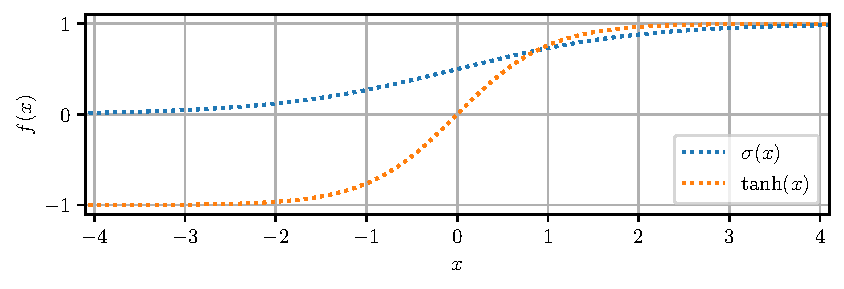
\includegraphics[width=0.9\textwidth]{own/sigmoid_tanh.pdf}
    \caption[
        The non-linear activation functions deployed within a standard GRU
    ]{
        The non-linear activation functions deployed within a standard GRU.
        The standard sigmoid function
        $\sigma (x) = \left(1 + e^{-x}\right)^{-1}$
        normalizes the values
        of the reset and update
        gate to the interval from zero to one
        (equation \ref{eq:gru_reset} and \ref{eq:gru_update}).
        The hyperbolic tangent
        $\tanh \left(x\right) = \left(e^x - e^{-x}\right)\left(e^x + e^{-x}\right)^{-1}$
        normalizes the values 
        of the candidate
        and, consequently, the hidden state 
        to the interval from minus to plus one
        (equation \ref{eq:gru_candidate} and \ref{eq:gru_layer_map_hidden}).
        \label{fig:gru_activations}}
\end{figure}


%\begin{figure}[h]
%    \centering
%    \subfloat[
%        Folded
%    ]{
%        \label{fig:rnn_folded}
%        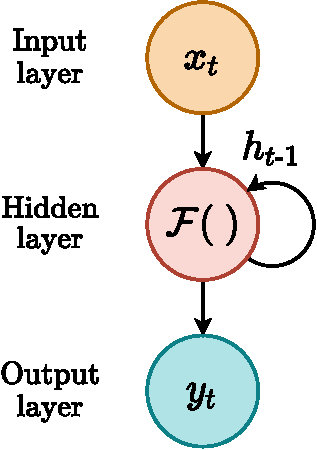
\includegraphics[height=0.35\textwidth]{own/rnn_folded.drawio.pdf}
%    }
%    \hspace*{2cm}                
%    \subfloat[
%        Unfolded
%    ]{
%        \label{fig:rnn_unfolded}
%        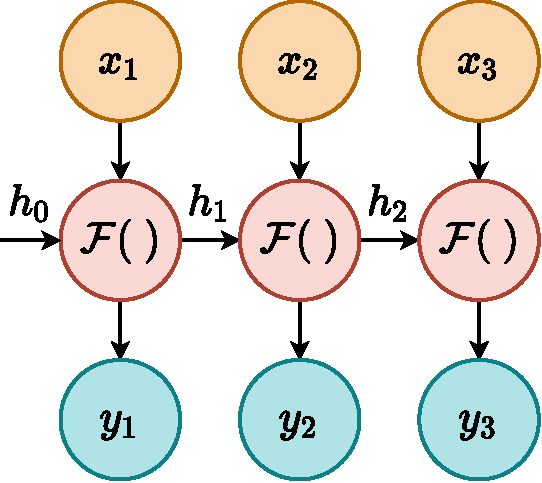
\includegraphics[height=0.35\textwidth]{own/rnn_unfolded.drawio.pdf}
%    }
%    \caption[
%        Folded and unfolded RNN
%    ]{
%        Folded schematic RNN with a single hidden layer 
%        that feeds the previous $h_{t-1}$ 
%        (or initial $h_{0}$) state  
%        back to the inference at the current time step $t$
%        and its time-unfolded representation
%        when processing the input of a time-series 
%        consisting of the three data points 
%        $\left(x_i\right)_{i\in\{1, 2, 3\}}$.
%
%        \label{fig:rnn_folded_unfolded}
%    }
%\end{figure}



\subsection*{Backpropagation through time}
The following presents the application 
of backpropagation through time
on a single integrated GRU layer
operating in many-to-one mode
in order to calculate
the gradients of the loss with respect to 
the GRU layer's trainable parameters.
During training,
these gradients are required
by gradient-based methods which update the trainable 
parameters with the target to minimize the loss.

%During training,
%the integrated GRU layers 
%of the ANN module of the navigation method of this thesis
%run in many-to-one mode,
%i.e., sequential inputs are mapped to single outputs \cite{ICE2020}.
%The trainable weights of the ANN module
%are updated with gradient-based methods 
%that minimize the loss.
%These gradient-based methods require 
%the knowledge of the gradient of the loss 
%with respect to the ANN's trainable parameters.
%The following paragraph shows the computation of these gradients 
%with backpropagation through time for 
%an integrated GRU layer in many-to-one mode.




%During the training of the ANN module 
%of the navigation method of this thesis
%(see section \ref{sec:ann_module}),
%the GRU sub-module,
%which integrates multiple, subsequent GRU layers,
%operates in many-to-one mode,
%i.e., the mapping of sequential inputs to single outputs.
%The following provides the theoretical
%background of training a single GRU layer in many-to-one mode.



%During the testing of the navigation method,
%the GRU layers of the ANN module operate 
%in one-to-one mode,
%i.e., a single input is mapped to a single output.
%At a high frequency,
%each incoming single data point,
%containing the current data from onboard sensors, 
%is mapped to a single navigation decision.
%During the training of the ANN module,
%on the contrary,
%the GRU layers process many-to-one,
%i.e., sequential input is mapped to a single output.
%The training data consist of sequences
%of data points labeled with a single navigation decision.
%The output of the gru layers is hence
%not the whole sequence of hidden states 
%but only the last infered hidden state of a sequence.
%This last hidden state is then forwarded
%through the remaining layers of the ANN module.
%Then,
%the final output of the ANN module
%is related with the label of the sequence
%in order to compute the loss.
%To update the weights of the network after an batch
%the loss is backpropagated.


Let a single GRU layer,
integrated into any superior ANN,
operate in many-to-one mode.
With biases enabled, 
the set of all structures 
that contain trainable parameters of the GRU layer
is aggregated from equation 
\ref{eq:gru_reset_params},
\ref{eq:gru_update_params} 
and \ref{eq:gru_candidate_params}
\begin{equation} \label{eq:gru_params}
    \Theta 
    = 
    \left\{  
        \underline{\underline A}^\text{r}_{x},
        \underline{b}^\text{r}_{x},
        \underline{\underline A}^\text{r}_{h},
        \underline{b}^\text{r}_{h},
        \underline{\underline A}^\text{u}_{x},
        \underline{b}^\text{u}_{x},
        \underline{\underline A}^\text{u}_{h},
        \underline{b}^\text{u}_{h},
        \underline{\underline A}^\text{c}_{x},
        \underline{b}^\text{c}_{x},
        \underline{\underline A}^\text{c}_{h},
        \underline{b}^\text{c}_{h}
    \right\}.
\end{equation}
The addition of the sizes of the structurs in the set $\Theta$
yields the total number of trainable parameters of the GRU layer
\begin{align}
    N^\text{param} 
    = 
    \begin{cases}
        3 N^\text{hidden} \left(
            N^\text{in}
            + N^\text{hidden}
            + 2
        \right)
        ,\ 
        & \text{if biases enabled} \\
        3 N^\text{hidden} \left(
            N^\text{in}
            + N^\text{hidden}
        \right)
        ,\ 
        & \text{else}.
    \end{cases}
\end{align}
At a single inference,
the GRU layer receives a batch of sequences of feature vectors
from the previous layer of the ANN
\begin{equation}
    \left(\underline x_t\right)_{t\in\{1,\dots,N^\text{seq}\},i}
    , \quad i \in \left\{1,\dots,N^\text{batch}\right\}.
\end{equation} 
The GRU layer in many-to-one mode maps each incoming batch of sequences
to a batch of single outputs,
whereby a single output is the hidden state lastly infered from a sequence
\begin{equation} \label{equ:gru_output_many_to_one}
    \underline y_i = \underline h_{N^{seq}, i},
    \quad i \in \left\{1,\dots,N^\text{batch}\right\}.
\end{equation}
The time-unfolded computation graph of the integrated GRU layer
for a single batch element is shown in figure \ref{fig:gru_unfolded}.
\begin{figure}
    \centering
    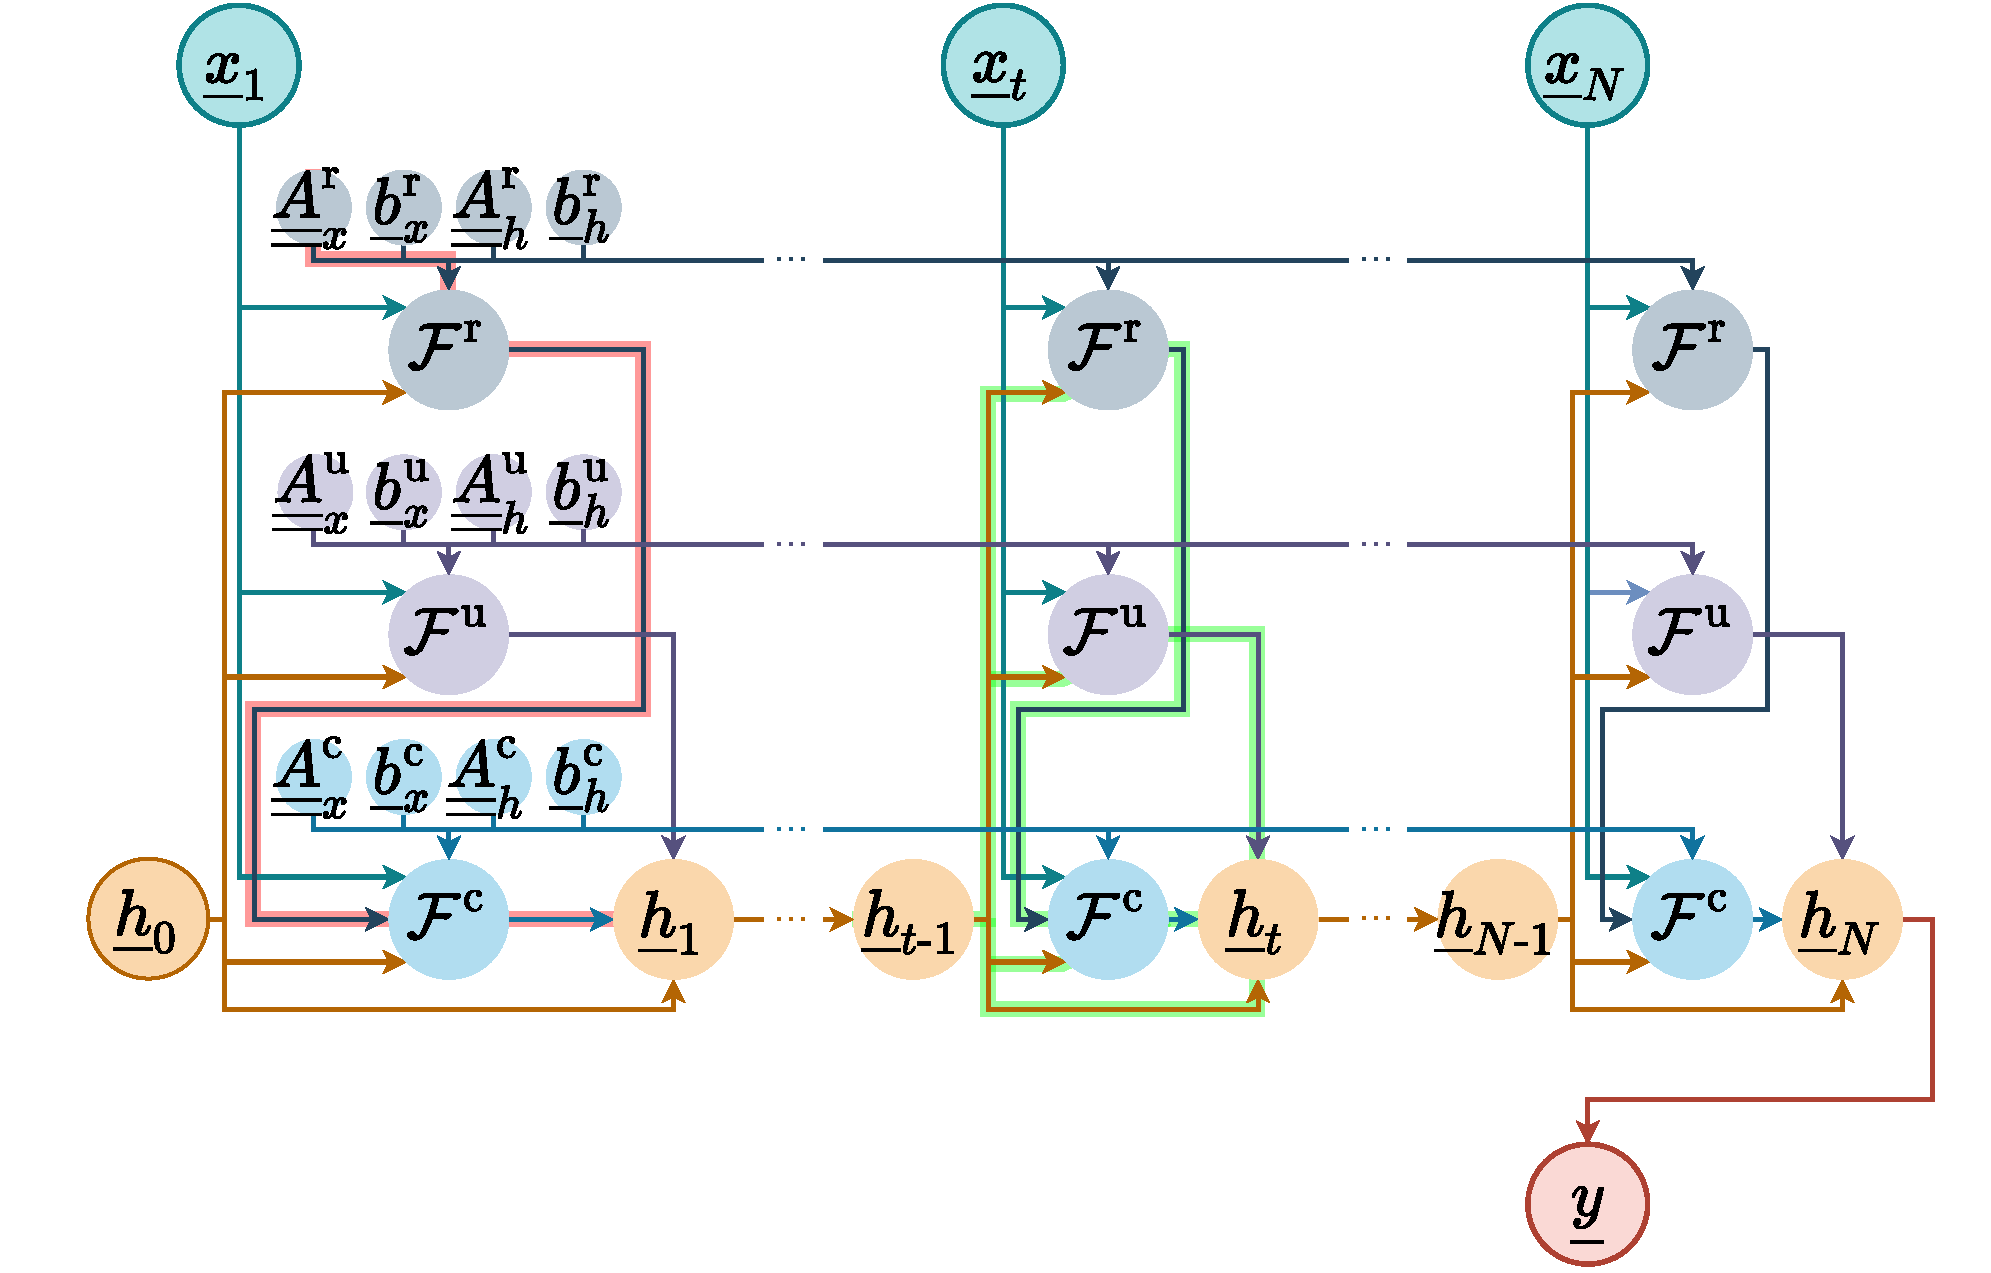
\includegraphics[width=0.9\textwidth]{own/gru_unfolded_intra_inter_paths.drawio.pdf}
    \caption[
        Time-unfolded computation graph of a GRU layer operating in many-to-one mode.
    ]{
        Time-unfolded computation graph of a GRU layer operating in many-to-one mode.
        The input sequence $\left(x_t\right)_{t\in\{1,\dots N\}}$ is mapped
        to the single output $\underline y$ which is equal to the lastly inferred, 
        hidden state $\underline h_N$.
        Equation \ref{eq:gru_reset}, \ref{eq:gru_update} and \ref{eq:gru_candidate}
        define the mapping to the 
        reset gate $\mathcal{F}^\text{r}$,
        update gate $\mathcal{F}^\text{u}$
        and candidate state $\mathcal{F}^\text{c}$, respectively.
        The hidden states 
        $\left(h_t\right)_{t\in\{1,\dots N\}}$
        are obtained with
        the mapping 
        $\mathcal{F}^\text{h}$ 
        defined by equation \ref{eq:gru_layer_map_hidden}
        whereas the initial hidden state $\underline h_0$ 
        (equation \ref{eq:gru_init_hidden_state})
        is defined by the user. 
        The trainable parameters 
        $\underline{\underline{A}}^\square_\square, \underline{b}^\square_\square$
        of the GRU layer
        are shared across all unfolded time steps.
        The backpropagation path of the intra-gradient with respect to 
        $\underline{\underline{A}}^\text{r}_x$
        (equation \ref{eq:gru_grad_intra_hidden_2_Arx}) is highlighted in red for the first time step $t=1$.
        The backpropagation paths of the inter-gradient 
        (equation \ref{eq:gru_grad_inter}) 
        is highlighted in green
        for the time step $t$.
        \label{fig:gru_unfolded}}
\end{figure}
The batches of single GRU outputs are forwarded to the subsequent layer of the ANN.
Whenever a batch has passed all the output layer of the ANN,
the loss $L$ of the batch is computed by averaging the losses of
the individual elements of the batch.
Because the seperate losses depend on their corresponding single GRU output,
the loss of the batch is a function of all of these outputs.
\begin{equation} \label{eq:loss_of_batch}
    L\left(\underline y_1, \dots, \underline y_{N^\text{batch}}\right) 
    = 
    \frac{1}{N^\text{batch}}
    \sum_{i=1}^{N^\text{batch}} L_i \left(\underline y_i\right).
\end{equation}
Gradient-based methods update the trainable parameters of the ANN
with the goal to minimize the loss of the batch.
For this, they require the knwoledge of the gradients of the loss 
with respect to the trainable parameters.
The update of the trainable parameters of the integrated GRU layer complies with
\begin{equation}
    \underset{\Theta}{\mathrm{argmin}}\ 
    L\left(\underline y_1, \dots, \underline y_{N^\text{batch}}\right).
\end{equation}
In conformity with Li \cite{li2016tutorial}, the gradient of the batch loss 
with respect to a single element
$\theta \in \Theta$ of the set of structures containing trainable parameters (equation \ref{eq:gru_params})
is computed based on backpropagation through time
\begin{align} \label{eq:gru_grad_loss_2_theta}
    &\frac{\partial}{\partial \theta}
        L\left(\underline y_1, \dots, \underline y_{N^\text{batch}}\right)
    \nonumber \\ & \quad \overset{\textcolor{blue}{(1)}}{=}
    \frac{1}{N^\text{batch}}
    \sum_{i=1}^{N^\text{batch}} 
    \frac{\partial}{\partial \theta}
    L_i \left(\underline y_i\right)
    \nonumber \\ & \quad \overset{\textcolor{blue}{(2)}}{=}
    \frac{1}{N^\text{batch}}
    \sum_{i=1}^{N^\text{batch}} \left(
        \frac{\partial L_i}{\partial \underline y_i}
        \frac{\partial \underline y_i}{\partial \theta}
    \right)
    \nonumber \\ & \quad \overset{\textcolor{blue}{(3)}}{=}
    \frac{1}{N^\text{batch}}
    \sum_{i=1}^{N^\text{batch}} \left[
        \frac{\partial L_i}{\partial \underline y_i}
        \sum_{j=1}^{N^{seq}} \left(
            \frac{\partial  \underline y_i}{\partial \underline h_{j, i}}
            \widehat{ \frac{\partial \underline h_{j, i}}{\partial \theta}}
        \right)
    \right]
    \nonumber \\ & \quad \overset{\textcolor{blue}{(4)}}{=}
    \frac{1}{N^\text{batch}}
    \sum_{i=1}^{N^\text{batch}} \left\{
        \frac{\partial L_i}{\partial \underline y_i}
        \sum_{j=1}^{N^{seq}} \left[
            \prod_{k=j+1}^{N^{seq}} \left(
                \frac{\partial \underline h_{k, i}}{\partial \underline h_{k-1, i}}
            \right)
            \widehat{ \frac{\partial \underline h_{j, i}}{\partial \theta}}
        \right]
    \right\}.
    \\[2ex]
        &\textcolor{blue}{\text{\footnotesize (1) 
            Loss of a batch (equ. \ref{eq:loss_of_batch})}} \nonumber \\
        &\textcolor{blue}{\text{\footnotesize (2) 
            Chain rule}} \nonumber \\
        &\textcolor{blue}{\text{\footnotesize (3) 
            Backpropagation through time (gradient $\widehat{\square}$ considers previous hidden states constant)}} \nonumber \\
        &\textcolor{blue}{\text{\footnotesize (4) 
            Many-to-one output (equ. \ref{equ:gru_output_many_to_one});
            chain rule applied on $\partial \underline y_i / \partial \underline h_{j, i}$}} \nonumber
\end{align}
In the above formula,
the gradient
$\widehat{\partial \underline h_{j, i} / \partial \theta}$,
hereinafter referred to as intra-gradient,
treats all previous hidden states 
$\underline h_{\tilde j,\dots, i}, \ \tilde j \in \{0, j-1\}$ as constants.
In doing so, the intra-gradient only covers 
the backpropagation path from 
the hidden state $\underline h_{j, i}$ to the 
parameter structure $\theta$
within the same time step $j$.
In order to compute the full gradient covering all backpropagation paths to $\theta$,
all intra-backpropagation paths are connected 
through time
to the GRU layer's output $\underline y _i$ 
by multiplying the intra-gradients with their corresponding chain of time step inter-gradients
$\partial \underline h_{k, i}/\partial \underline h_{k-1, i}$.
For demonstration purposes,
the intra-gradient with respect to 
$\theta=\underline{\underline{A}}^\text{r}_x$ 
(the corresponding backpropagation path is highlighted for the first time step in figure \ref{fig:gru_unfolded})
is examplarily derived as
\begin{align} \label{eq:gru_grad_intra_hidden_2_Arx}
    \widehat{\frac{\partial \underline h_{t, i}}{\partial \underline{\underline{A}}^\text{r}_x}}
    &\overset{\textcolor{blue}{(1)}}{=}
    \widehat{\frac{\partial}{\partial \underline{\underline{A}}^\text{r}_x}} \left\{
        \left[
            \underline 1 
            -
            \mathcal{F}^\text{u}\left(\chi\right)
        \right]
        \odot
        \mathcal{F}^\text{c} \left(\chi\right)
        +
        \mathcal{F}^\text{u}\left(\chi\right)
        \odot
        \underline h_{t\text -1,i}
    \right\}
    %\nonumber \\ & \quad \overset{\textcolor{blue}{(2)}}{=}
    \nonumber \\ &\overset{\textcolor{blue}{(2)}}{=}
    \mathrm{diag} \left[
        \underline 1 
        -
        \mathcal{F}^\text{u}\left(\chi\right)
    \right]
    \widehat{
        \frac{\partial \mathcal{F}^\text{c} \left(\chi\right)}
            {\partial \underline{\underline{A}}^\text{r}_x} 
    }
    \\[2ex]
    &\textcolor{blue}{\text{\footnotesize (1) 
            Mapping to hidden state (equ. \ref{eq:gru_layer_current_hidden}, \ref{eq:gru_layer_map_hidden}); 
            $\chi :=  \left(\underline x_{t, i}, \underline h_{t\text{-}1, i}\right)$}} \nonumber \\
    &\textcolor{blue}{\text{\footnotesize (2) 
        Sum rule of differentiation;
    }} \nonumber \\
    &\textcolor{blue}{\text{\footnotesize \qquad
        Mapping to update gate (equ. \ref{eq:gru_update}): 
        $\widehat{\partial \mathcal{F}^\text{u} / \partial \underline{\underline{A}}^\text{r}_x} = 0$ 
    }} \nonumber \\
    &\textcolor{blue}{\text{\footnotesize \qquad
        Consider previous hidden states constant: 
        $\widehat{\partial \underline h_{t\text -1, i} / \partial \underline{\underline{A}}^\text{r}_x} = 0$;
    }} \nonumber \\
    &\textcolor{blue}{\text{\footnotesize \qquad
        Hadamard product of two vectors (equ. \ref{eq:hadamard_product_two_vectors})
    }} \nonumber
\end{align}
with
\begin{align} \label{eq:gru_grad_intra_candidate_2_Arx}
    \widehat{
        \frac{\partial \mathcal{F}^\text{c} \left(\chi\right)}
            {\partial \underline{\underline{A}}^\text{r}_x}
    }
    & \overset{\textcolor{blue}{(1)}}{=}
    \widehat{
        \frac{\partial}{\partial \underline{\underline{A}}^\text{r}_x} 
    }
    \left\{
        \overset{\scriptscriptstyle \odot}{\tanh} \left[
            \underbrace{
            \underline{\underline A}^\text{c}_{x}
            \underline x_{t,i}
            +
            \underline b^\text{c}_{x}
            +
            \mathcal{F}^\text{r}\left(\underline x_{t, i}, \underline h_{t\text -1, i}\right)
            \odot
            \left(
                \underline{\underline A}^\text{c}_{h}
                \underline h_{t\text -1,i}
                +
                \underline b^\text{c}_{h}
            \right)}_{:=\chi^\text{c}}
        \right]
    \right\}
    \nonumber \\ & \overset{\textcolor{blue}{(2)}}{=}
    \mathrm{diag} \left[
        \frac{\partial}{\partial \chi^\text{c}}
        \overset{\scriptscriptstyle \odot}{\tanh} \left(\chi^\text{c}\right)
    \right] 
    \cdot 
    \widehat{
        \frac{\partial \chi^\text{c}}
            {\partial \underline{\underline{A}}^\text{r}_x} 
    }
    \nonumber \\ & \overset{\textcolor{blue}{(3)}}{=}
    \mathrm{diag} \left[
        1 - \overset{\scriptscriptstyle \odot}{\tanh}{}^2 \left(\chi^\text{c}\right)
    \right] 
    \cdot
    \mathrm{diag} \left(
        \underline{\underline A}^\text{c}_{h}
        \underline h_{t-1,i}
        +
        \underline b^\text{c}_{h}
    \right)
    \widehat{
        \frac{\partial \mathcal{F}^\text{r}\left(\underline x_{t, i}, \underline h_{t\text -1, i}\right)}
            {\partial \underline{\underline{A}}^\text{r}_x} 
    }
    \\[2ex]
    &\textcolor{blue}{\text{\footnotesize (1) 
            Mapping to candidate state (equ. \ref{eq:gru_candidate}); 
            $\chi :=  \left(\underline x_{t, i}, \underline h_{t\text{-}1, i}\right)$}} \nonumber \\
    &\textcolor{blue}{\text{\footnotesize (2) 
        Chain rule of differentiation;  
    }} \nonumber \\
    &\textcolor{blue}{\text{\footnotesize \qquad
        Derivative of function applied element-wise on vector
        (equ. \ref{eq:derivative_vector_elementwise_applied_function})
    }} \nonumber \\
    &\textcolor{blue}{\text{\footnotesize (3) 
        Derivative of hyperbolic tangent (equ. \ref{eq:derivative_tanh}); 
    }} \nonumber \\
    &\textcolor{blue}{\text{\footnotesize \qquad
    Hadamard product of two vectors (equ. \ref{eq:hadamard_product_two_vectors})
    }} \nonumber
\end{align}
and
\begin{align} \label{eq:gru_grad_intra_reset_2_Arx} 
    \widehat{
        \frac{\partial \mathcal{F}^\text{r}\left(\underline x_{t, i}, \underline h_{t\text -1, i}\right)}
            {\partial \underline{\underline{A}}^\text{r}_x} 
    }
    &\overset{\textcolor{blue}{(1)}}{=}
    \widehat{
        \frac{\partial}{\partial \underline{\underline{A}}^\text{r}_x} 
    }
    \left[
        \overset{\scriptscriptstyle \odot}{\sigma} \left(
            \underbrace{
            \underline{\underline A}^\text{r}_{x}
            \underline x_{t,i}
            +
            \underline b^\text{r}_{x}
            +
            \underline{\underline A}^\text{r}_{h}
            \underline h_{t\text -1,i}
            +
            \underline b^\text{r}_{h}}_{:=\chi^\text{r}}
        \right)
    \right]
    \nonumber \\ & \overset{\textcolor{blue}{(2)}}{=}
    \mathrm{diag} \left[
        \frac{\partial}{\partial \chi^\text{r}}
        \overset{\scriptscriptstyle \odot}{\sigma} \left(\chi^\text{r}\right)
    \right]
    \cdot
    \widehat{
        \frac{\partial \chi^\text{u}{}}
            {\partial \underline{\underline{A}}^\text{r}_x} 
    }
    \nonumber \\ & \overset{\textcolor{blue}{(3)}}{=}
    \mathrm{diag} \left\{
        \overset{\scriptscriptstyle \odot}{\sigma} \left(\chi^\text{r}\right)
        \odot
        \left[
            1 -  \overset{\scriptscriptstyle \odot}{\sigma} \left(\chi^\text{r}\right)
        \right]
    \right\}
    \cdot
    \frac{\partial \underline{\underline A}^\text{r}_{x}\underline x_{t,i}}
        {\partial \underline{\underline{A}}^\text{r}_x} 
        .
    \\[2ex]
        &\textcolor{blue}{\text{\footnotesize (1) 
            Mapping to reset gate (equ. \ref{eq:gru_reset})}} \nonumber \\
        &\textcolor{blue}{\text{\footnotesize (2) 
            Chain rule of differentiation;
        }} \nonumber \\
        &\textcolor{blue}{\text{\footnotesize \qquad
            Derivative of function applied element-wise on vector
            (equ. \ref{eq:derivative_vector_elementwise_applied_function})
        }} \nonumber \\
        &\textcolor{blue}{\text{\footnotesize (3) 
            Derivative of sigmoid function (equ. \ref{eq:derivative_sigmoid})
        }} \nonumber
\end{align}
For the computation of the gradient
$\partial \left(\underline{\underline A}^\text{r}_{x}\underline x_{t,i}\right)
        /\partial \underline{\underline{A}}^\text{r}_x
$,
which is a 3-dimensional matrix
whose information content is only 2-dimensional,
refer to \cite{LearnedMiller}, for example.



The in equation \ref{eq:gru_grad_loss_2_theta} required inter-gradient
(the corresponding backpropagation path is highlighted in figure \ref{fig:gru_unfolded})
, i.e., 
the gradient of the current hidden state with respect to the previous hidden state,
is derived as
%$\underline h_{t, i} = 
%\mathcal{F}^\text{h} \left(\underline x_{t, i}, \underline h_{t\text{-}1, i}\right)$
%and 
%$\chi :=  \left(\underline x_{t, i}, \underline h_{t\text{-}1, i}\right)$:
\begin{align} \label{eq:gru_grad_inter}
    \frac{\partial \underline h_{t, i}}{\partial \underline h_{t\text{-}1, i}}
    %\nonumber \\ & \quad \overset{\textcolor{blue}{(1)}}{=}
    %\frac{\partial}{\partial \underline h_{t\text{-}1, i}}
    %\mathcal{F}^\text{h} \left(\underline x_{t, i}, \underline h_{t\text{-}1, i}\right)
    %\nonumber \\ & \quad \overset{\textcolor{blue}{(1)}}{=}
    &\overset{\textcolor{blue}{(1)}}{=}
    \frac{\partial}{\partial \underline h_{t\text{-}1, i}} \left\{
        \left[
            \underline 1 
            -
            \mathcal{F}^\text{u}\left(\chi\right)
        \right]
        \odot
        \mathcal{F}^\text{c} \left(\chi\right)
        +
        \mathcal{F}^\text{u}\left(\chi\right)
        \odot
        \underline h_{t\text -1,i}
    \right\}
    %\nonumber \\ & \quad \overset{\textcolor{blue}{(2)}}{=}
    \nonumber \\ &\overset{\textcolor{blue}{(2)}}{=}
    \frac{\partial}{\partial \underline h_{t\text{-}1, i}} \left\{
        \left[
            \underline 1 
            -
            \mathcal{F}^\text{u}\left(\chi\right)
        \right]
        \odot
        \mathcal{F}^\text{c} \left(\chi\right)
    \right\}
    +
    \frac{\partial}{\partial \underline h_{t\text{-}1, i}} \left\{
        \mathcal{F}^\text{u}\left(\chi\right)
        \odot
        \underline h_{t-1,i}
    \right\}
    %\nonumber \\ & \quad \overset{\textcolor{blue}{(3)}}{=}
    \nonumber \\ & \overset{\textcolor{blue}{(3)}}{=}
    - \mathrm{diag}\left[\mathcal{F}^\text{c} \left(\chi\right)\right] 
    \frac{\partial \mathcal{F}^\text{u}\left(\chi\right)}
        {\partial \underline h_{t\text{-}1, i}}
    +
    \mathrm{diag} \left[
        \underline 1 
        -
        \mathcal{F}^\text{u}\left(\chi\right)
    \right]
    \frac{\partial \mathcal{F}^\text{c} \left(\chi\right)}
        {\partial \underline h_{t\text{-}1, i}}
    \nonumber \\ &\qquad +
    \mathrm{diag} \left(\underline h_{t-1,i}\right)
    \frac{\partial \mathcal{F}^\text{u}\left(\chi\right)}
        {\partial \underline h_{t\text{-}1, i}}
    +
    \mathrm{diag} \left[
        \mathcal{F}^\text{u}\left(\chi\right)
    \right].
    \\[2ex]
    &\textcolor{blue}{\text{\footnotesize (1) 
            Mapping to current hidden state (equ. \ref{eq:gru_layer_current_hidden}, \ref{eq:gru_layer_map_hidden}); 
            $\chi :=  \left(\underline x_{t, i}, \underline h_{t\text{-}1, i}\right)$}} \nonumber \\
    &\textcolor{blue}{\text{\footnotesize (2) 
        Sum rule of differentiation
    }} \nonumber \\
    &\textcolor{blue}{\text{\footnotesize (3) 
        Differentiation of Hadamard product of two vectors 
        (equ. \ref{eq:differentiation_hadamard_product_two_vectors})
    }} \nonumber
\end{align}
The in equation \ref{eq:gru_grad_inter} required gradient 
of the current update gate with respect to the previous hidden state is derived as 
\begin{align} \label{eq:gru_grad_update_2_previous_hidden} 
    \frac{\partial
    \mathcal{F}^\text{u} \left(\underline x_{t, i}, \underline h_{t\text{-}1, i}\right)
    }{\partial \underline h_{t\text{-}1, i}}
    &\overset{\textcolor{blue}{(1)}}{=}
    \frac{\partial}{\partial \underline h_{t\text{-}1, i}}
    \left[
        \overset{\scriptscriptstyle \odot}{\sigma} \left(
            \underbrace{
            \underline{\underline A}^\text{u}_{x}
            \underline x_{t,i}
            +
            \underline b^\text{u}_{x}
            +
            \underline{\underline A}^\text{u}_{h}
            \underline h_{t\text -1,i}
            +
            \underline b^\text{u}_{h}}_{:=\chi^\text{u}}
        \right)
    \right]
    \nonumber \\ & \overset{\textcolor{blue}{(2)}}{=}
    \mathrm{diag} \left[
        \frac{\partial}{\partial \chi^\text{u}}
        \overset{\scriptscriptstyle \odot}{\sigma} \left(\chi^\text{u}\right)
    \right]
    \cdot \frac{\partial}{\partial \underline h_{t\text{-}1, i}} \chi^\text{u}{}
    \nonumber \\ & \overset{\textcolor{blue}{(3)}}{=}
    \mathrm{diag} \left\{
        \overset{\scriptscriptstyle \odot}{\sigma} \left(\chi^\text{u}\right)
        \odot
        \left[
            1 -  \overset{\scriptscriptstyle \odot}{\sigma} \left(\chi^\text{u}\right)
        \right]
    \right\}
    \cdot \underline{\underline A}^\text{u}_{h}.
    \\[2ex]
        &\textcolor{blue}{\text{\footnotesize (1) 
            Mapping to update gate (equ. \ref{eq:gru_update})}} \nonumber \\
        &\textcolor{blue}{\text{\footnotesize (2) 
            Chain rule of differentiation;
        }} \nonumber \\
        &\textcolor{blue}{\text{\footnotesize \qquad
            Derivative of function applied element-wise on vector
            (equ. \ref{eq:derivative_vector_elementwise_applied_function})
        }} \nonumber \\
        &\textcolor{blue}{\text{\footnotesize (3) 
            Derivative of sigmoid function (equ. \ref{eq:derivative_sigmoid})
        }} \nonumber
\end{align}
The in equation \ref{eq:gru_grad_inter} 
required gradient of the current candidate state
with respect to the previous hidden state is derived as 
\begin{align} \label{eq:gru_grad_candidate_2_previous_hidden}
    &\frac{\partial}{\partial \underline h_{t\text{-}1, i}}
    \mathcal{F}^\text{c}\left(\underline x_{t, i}, \underline h_{t\text -1, i}\right)
    \nonumber \\ & \quad \overset{\textcolor{blue}{(1)}}{=}
    \frac{\partial}{\partial \underline h_{t\text{-}1, i}}
    \left\{
        \overset{\scriptscriptstyle \odot}{\tanh} \left[
            \underbrace{
            \underline{\underline A}^\text{c}_{x}
            \underline x_{t,i}
            +
            \underline b^\text{c}_{x}
            +
            \mathcal{F}^\text{r}\left(\underline x_{t, i}, \underline h_{t\text -1, i}\right)
            \odot
            \left(
                \underline{\underline A}^\text{c}_{h}
                \underline h_{t\text -1,i}
                +
                \underline b^\text{c}_{h}
            \right)}_{:=\chi^\text{c}}
        \right]
    \right\}
    \nonumber \\ & \quad \overset{\textcolor{blue}{(2)}}{=}
    \mathrm{diag} \left[
        \frac{\partial}{\partial \chi^\text{c}}
        \overset{\scriptscriptstyle \odot}{\tanh} \left(\chi^\text{c}\right)
    \right] 
    \cdot 
    \frac{\partial}{\partial \underline h_{t\text{-}1, i}} \chi^\text{c}
    \nonumber \\ & \quad \overset{\textcolor{blue}{(3)}}{=}
    \mathrm{diag} \left[
        1 - \overset{\scriptscriptstyle \odot}{\tanh}{}^2 \left(\chi^\text{c}\right)
    \right] 
    \nonumber \\ &\quad \quad  \cdot
    \left\{
        \mathrm{diag} \left(
            \underline{\underline A}^\text{c}_{h}
            \underline h_{t-1,i}
            +
            \underline b^\text{c}_{h}
        \right)
        \frac{\partial \mathcal{F}^\text{r}\left(\underline x_{t, i}, \underline h_{t\text -1, i}\right)}
        {\partial \underline h_{t\text -1, i}}
        +
        \mathrm{diag}\left[
            \mathcal{F}^\text{r}\left(\underline x_{t, i}, \underline h_{t\text -1, i}\right)
        \right]
        \underline{\underline A}^\text{c}_{h}
    \right\}.
    \\[2ex]
        &\textcolor{blue}{\text{\footnotesize (1)
            Mapping to candidate state (equ. \ref{eq:gru_candidate})
        }} \nonumber \\
        &\textcolor{blue}{\text{\footnotesize (2) 
            Chain rule of differentiation;  
        }} \nonumber \\
        &\textcolor{blue}{\text{\footnotesize \qquad 
            Derivative of function applied element-wise on vector
            (equ. \ref{eq:derivative_vector_elementwise_applied_function})
        }} \nonumber \\
        &\textcolor{blue}{\text{\footnotesize (3) 
            Derivative of hyperbolic tangent (equ. \ref{eq:derivative_tanh}); 
        }} \nonumber \\
        &\textcolor{blue}{\text{\footnotesize \qquad
            Differentiation of Hadamard product of two vectors 
            (equ. \ref{eq:differentiation_hadamard_product_two_vectors})
        }} \nonumber
\end{align}
The in equation \ref{eq:gru_grad_candidate_2_previous_hidden} 
required gradient of the current reset gate
with respect to the previous hidden state shares the same structure
with the gradient of equation \ref{eq:gru_grad_update_2_previous_hidden} 
and is hence derived as
\begin{align}
    \frac{\partial}{\partial \underline h_{t\text{-}1, i}}
    \mathcal{F}^\text{r} \left(\underline x_{t, i}, \underline h_{t\text{-}1, i}\right)
    &=
    \mathrm{diag} \left\{
        \overset{\scriptscriptstyle \odot}{\sigma} \left(\chi^\text{r}\right)
        \odot
        \left[
            1 -  \overset{\scriptscriptstyle \odot}{\sigma} \left(\chi^\text{r}\right)
        \right]
    \right\}
    \cdot \underline{\underline A}^\text{r}_{h}
    \nonumber \\
    \text{with } \chi^\text{r} & :=
    \underline{\underline A}^\text{r}_{x}
            \underline x_{t,i}
            +
            \underline b^\text{r}_{x}
            +
            \underline{\underline A}^\text{r}_{h}
            \underline h_{t\text -1,i}
            +
            \underline b^\text{r}_{h}.
\end{align}
The above derivations revert to the following equations.
Equations (4.5.73) and (4.5.17) of Abramowitz and Stegun \cite{D.1966}
yield the derivative of the hyperbolic tangent as
\begin{equation} \label{eq:derivative_tanh}
    \frac{\text d}{\text d x} \tanh (x) = 1 - \tanh^2 (x).
\end{equation}
The derivative of the sigmoid function (e.g., \cite{Minai1993})
is given by
\begin{equation} \label{eq:derivative_sigmoid}
    \frac{\text d}{\text d x} \sigma \left(x\right) 
    = 
    \sigma \left(x\right) 
    \left[
        1 - \sigma \left(x\right)
    \right].
\end{equation}
The hadamard product of two vectors can be reformulated as the
matrix product of a diagonal matrix and a vector \cite{Brookes2020}
\begin{equation} \label{eq:hadamard_product_two_vectors}
    \underline x_1 \odot \underline x_2 
= 
    \mathrm{diag} \left(\underline x_1\right) \underline x_2 
=   
    \mathrm{diag} \left(\underline x_2\right) \underline x_1.
\end{equation}
Together with the product rule of differentiation, the derivative of the Hadamard product of two vectors 
is therewith identified as
\begin{equation} \label{eq:differentiation_hadamard_product_two_vectors}
    \frac{\partial}{\partial t} \left(
        \underline x_1 \odot \underline x_2 
    \right)
    =   
    \mathrm{diag} \left(\underline x_2\right)
    \frac{\partial \underline x_1}{\partial t} 
    +
    \mathrm{diag} \left(\underline x_1\right)
    \frac{\partial \underline x_2}{\partial t}.
\end{equation}
The derivative of a function
$f:\mathbb{R}\rightarrow\mathbb{R}$, that is applied element-wise on a vector $\underline x$,
is the diagonal matrix built from the derivative of the function applied element-wise on the vector
\begin{equation} \label{eq:derivative_vector_elementwise_applied_function}
        \frac{\partial}{\partial \underline x} 
        \overset{\scriptscriptstyle \odot}{f} \left(
                \underline x
            \right)
    =
        \mathrm{diag} \left[
            \overset{\scriptscriptstyle \odot}{f'}  \left(
                \underline x
            \right)
        \right].
\end{equation}
The above statement can be derived 
from the calculation of the differential of the function
\begin{align}
    &\frac{\text d}{\text d \underline x}
    \overset{\scriptscriptstyle \odot}{f} \left(
        \underline x
    \right)
    \cdot \text d \underline x
\overset{\textcolor{blue}{(1)}}{=}
    \text d 
    \overset{\scriptscriptstyle \odot}{f} \left(
        \underline x
    \right)
\overset{\textcolor{blue}{(2)}}{=}
    \left[
        \overset{\scriptscriptstyle \odot}{f'}  \left(
            \underline x
        \right)
    \right]
    \odot \text d \underline x
\overset{\textcolor{blue}{(3)}}{=}
    \mathrm{diag} \left[
        \overset{\scriptscriptstyle \odot}{f'}  \left(
            \underline x
        \right)
    \right]\cdot
    \text d \underline x.
    \\[2ex]
        &\quad\textcolor{blue}{\text{\footnotesize (1) Relation of differential and derivative}} \nonumber \\
        &\quad\textcolor{blue}{\text{\footnotesize (2) Chain rule element-wise applied}} \nonumber \\
        &\quad\textcolor{blue}{\text{\footnotesize (3) Hadamard product of two vectors (equ. \ref{eq:hadamard_product_two_vectors})}}
\end{align}